% Latex template: mahmoud.s.fahmy@students.kasralainy.edu.eg
% For more details: https://www.sharelatex.com/learn/Beamer

\documentclass{beamer}					% Document class

\setbeamertemplate{footline}[text line]{%
  \parbox{\linewidth}{\vspace*{-8pt}A brief introduction to deep generative models\hfill\insertshortauthor\hfill\insertpagenumber}}
\setbeamertemplate{navigation symbols}{}

\usepackage[english]{babel}				% Set language
\usepackage[utf8x]{inputenc}			% Set encoding

\mode<presentation>						% Set options
{
  \usetheme{default}					% Set theme
  \usecolortheme{default} 				% Set colors
  \usefonttheme{default}  				% Set font theme
  \setbeamertemplate{caption}[numbered]	% Set caption to be numbered
}

% Uncomment this to have the outline at the beginning of each section highlighted.
%\AtBeginSection[]
%{
%  \begin{frame}{Outline}
%    \tableofcontents[currentsection]
%  \end{frame}
%}

\usepackage{graphicx}					% For including figures
\usepackage{booktabs}					% For table rules
\usepackage{hyperref}					% For cross-referencing

\title{A brief introduction to deep generative models}	% Presentation title
\author{Clayton W. Seitz}								% Presentation author
\date{\today}									% Today's date	

\begin{document}

% Title page
% This page includes the informations defined earlier including title, author/s, affiliation/s and the date
\begin{frame}
  \titlepage
\end{frame}

% Outline
% This page includes the outline (Table of content) of the presentation. All sections and subsections will appear in the outline by default.
\begin{frame}{Outline}
  \tableofcontents
\end{frame}

% The following is the most frequently used slide types in beamer
% The slide structure is as follows:
%
%\begin{frame}{<slide-title>}
%	<content>
%\end{frame}


\section{Generative Models}

\begin{frame}{The logic of generative modeling}

Say we have a set of variables $\mathbf{x} = (x_{1},x_{2},...,x_{n})$ which might have some statistical dependence\\
\vspace{0.1in}
The variable $\mathbf{x}$ might be an amino acid sequence, gene expression data, microscopy image, etc.\\
\vspace{0.1in}
\begin{itemize}
\item Often we are handed a batch of empirical samples $\{\mathbf{x}_{i}\}_{i=1}^{N}$
\item We want to know the generating distribution $p(\mathbf{x})$
\end{itemize}

In supervised \textcolor{red}{generative learning}, we try to explicity learn the joint distribution $p(\mathbf{x}) = \prod_{i=1}^{N-1}p(x_{i}|x_{i+1:N})p(x_{N})$, which is generally more difficult than discriminative learning. 

\end{frame}


\begin{frame}{Perks of generative modeling}

\begin{itemize}
\item Fitting complete multivariate distributions $p(\mathbf{x})$ goes beyond correlation-based or clustering approaches
\item Correlations cannot discover partial correlation in the context of other neighbors
\item Fitting $p(\mathbf{x})$ permits sampling based inference
\end{itemize}

\end{frame}

\begin{frame}{Why generative modeling is difficult}

When describing a distribution over multiple variables, we may not know the proper normalization $Z$. That is,

\begin{equation*}
p(\mathbf{x}) = \frac{1}{Z}\tilde{p}(\mathbf{x})
\end{equation*}

\vspace{0.1in}
This \textcolor{red}{very important} situation arises in several contexts:\\
\vspace{0.1in}
1. In \textcolor{red}{Bayesian inference} where $p(x_{1}|x_{2}) = p(x_{2}|x_{1})p(x_{1})/p(x_{2})$ is intractable due to $Z = p(x_{2}) = \int p(x_{2}|x_{1})p(x_{1})dx_{1}$. This integral can be very difficult or impossible to
compute.\\
\vspace{0.1in}
2. In models from statistical physics, e.g. the Ising model, we only know
$\tilde{p}(\mathbf{x}) = e^{−H(\mathbf{x})}$ where $H(\mathbf{x})$ is the Hamiltonian

\end{frame}

\begin{frame}{Variational autoencoders (VAEs)}
A variational solution to generative modeling

\begin{center}
\begin{figure}
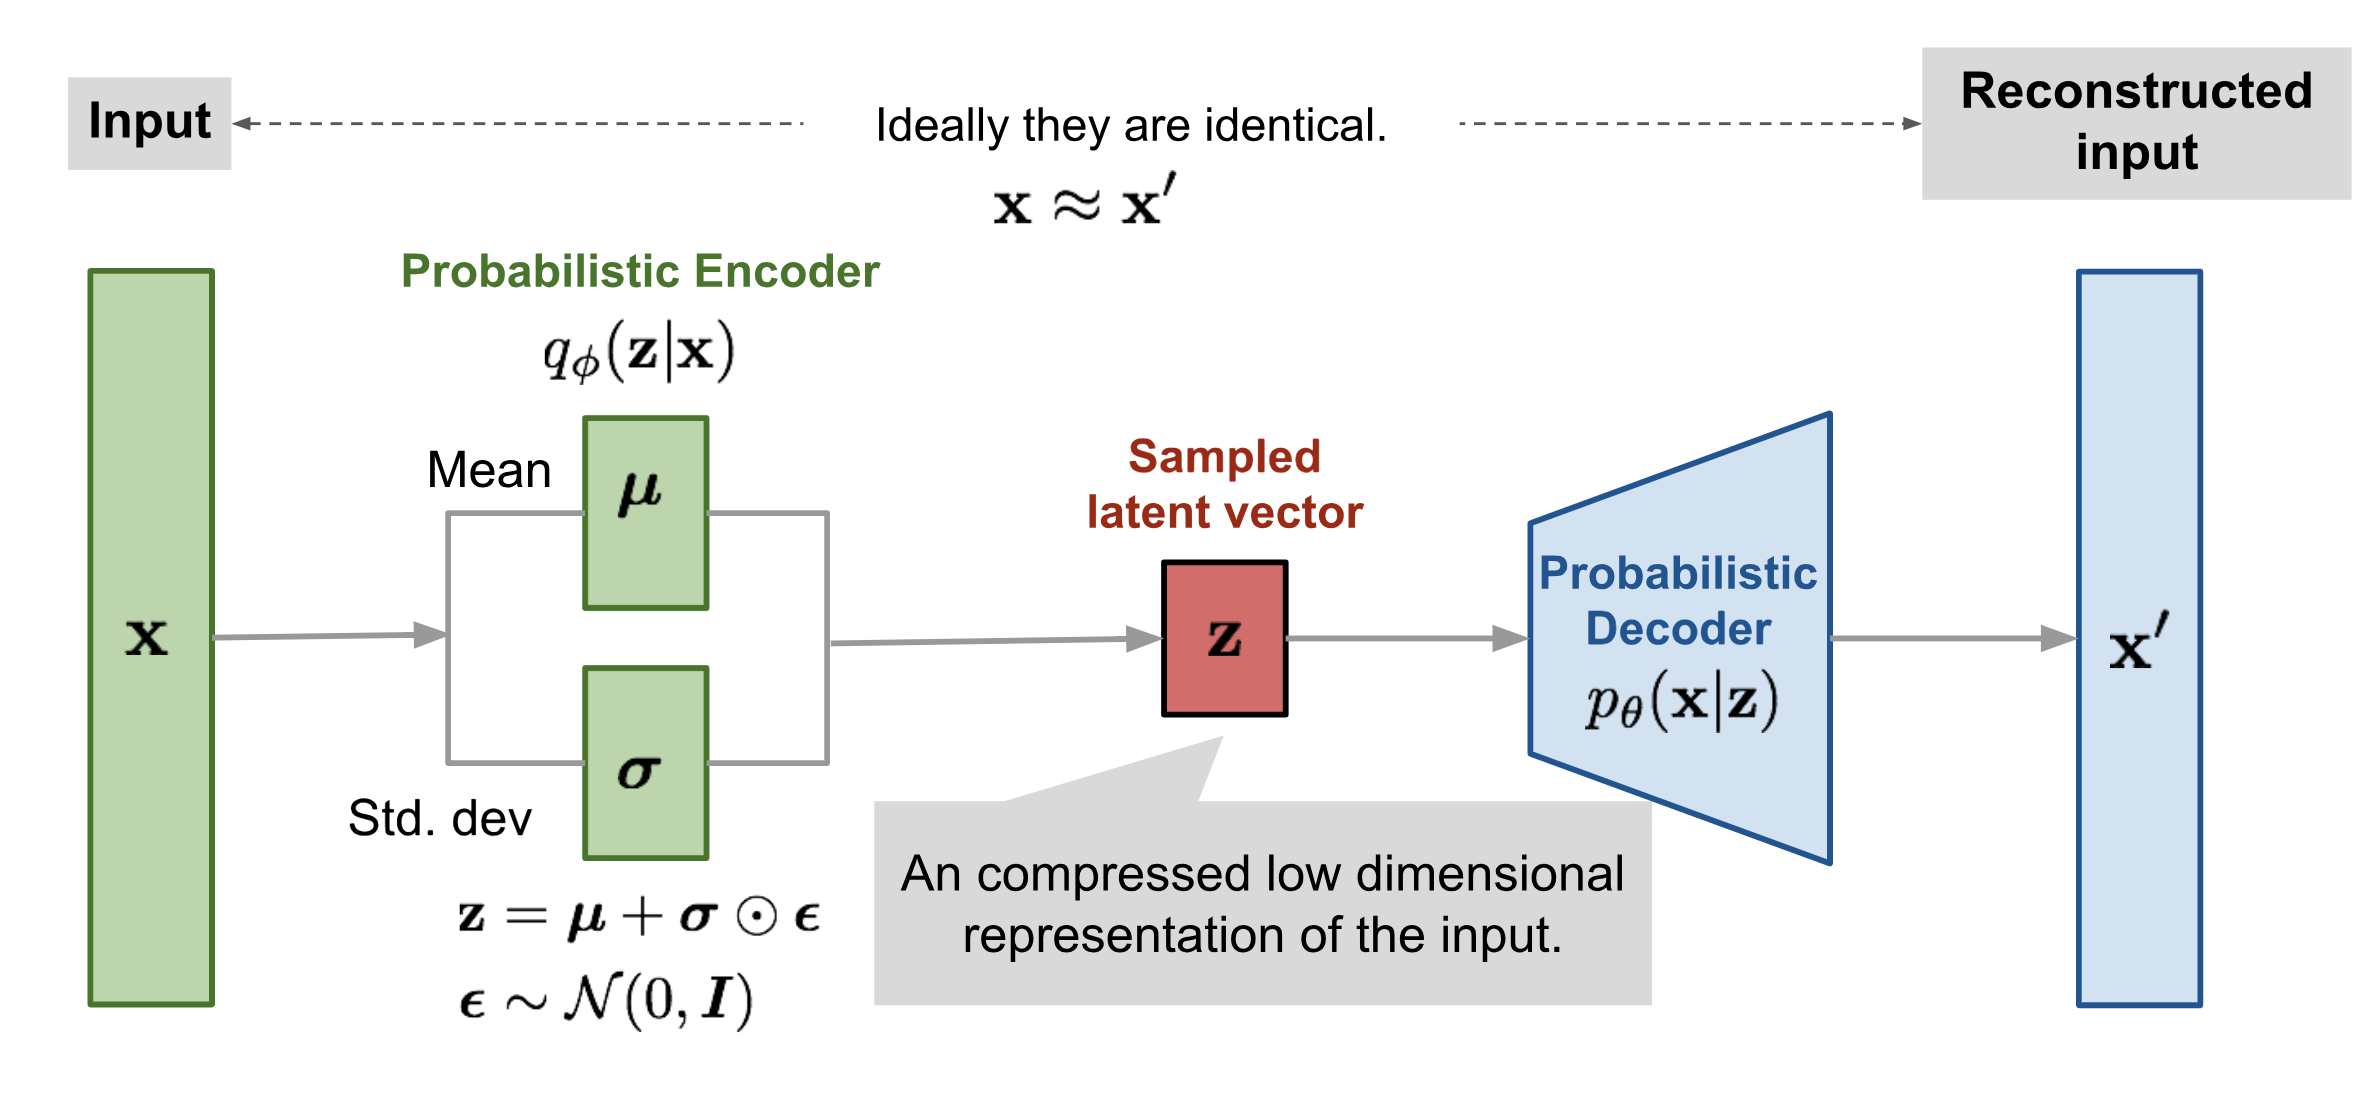
\includegraphics[width=0.9\textwidth]{vae}
\caption{\textbf{Variational autoencoder architecture} Taken from Lopez 2020 in EMBO}
\end{figure}
\end{center}
\end{frame}


\begin{frame}{Bayesian inference}

The variable $\mathbf{x}$ has a latent representation or code $\mathbf{z}$. We often say that $\mathbf{z}$ is the \emph{causal source} of $\mathbf{x}$. Ultimately, we would like to know the distribution $P_{\Phi}(\mathbf{x})$

\begin{equation*}
P_{\phi}(\mathbf{x}) = \frac{P_{\phi}(\mathbf{x|z})P_{\phi}(\mathbf{z})}{Q_{\psi}(\mathbf{z|x})}
\end{equation*}

in order to find the model parameters that maximize the likelihood of the observed data:

\begin{equation*}
\Phi^{*} = \underset{\Phi}{\mathrm{argmin}} -\log P_{\Phi}(\mathbf{x}) 
\end{equation*}

but we generally do not know $P_{\psi}(\mathbf{z|x})$ due to the intractable integral $Z = \int P_{\phi}(\mathbf{x|z})P_{\phi}(\mathbf{z})d\mathbf{z}$ (see slide 5)

\end{frame}

\begin{frame}{Computing the evidence}

We can rewrite the evidence as

\begin{align*}
P_{\phi}(\mathbf{x}) &= \int P_{\phi}(\mathbf{z})P_{\phi}(\mathbf{x|z})d\mathbf{z}\\
&= \int P_{\phi}(\mathbf{z})P_{\phi}(\mathbf{x|z})\frac{P_{\phi}(\mathbf{z|x})}{P_{\phi}(\mathbf{z|x})}d\mathbf{z}\\
&= \mathbb{E}_{\mathbf{z}\sim P_{\phi}(\mathbf{z|x})} \frac{P_{\phi}(\mathbf{z})P_{\phi}(\mathbf{x|z})}{P_{\phi}(\mathbf{z|x})}
\end{align*}

where $P_{\phi}(\mathbf{z|x})$ is our model "encoder"

\end{frame}

\begin{frame}{The evidence lower bound}

\begin{align*}
\log P_{\phi}(\mathbf{x}) &= \log \int_{z}P(x,z)dx\\
&= \log \int_{z} P(x,z)\frac{Q(z|x)}{Q(z|x)}dz\\
&= \log \mathbb{E}_{\mathbf{z}\sim P_{\phi}(\mathbf{z|x})} \frac{P(x|z)P(z)}{Q(z|x)}\\
&\geq \mathbb{E}_{\mathbf{z}\sim P_{\phi}(\mathbf{z|x})} \log \frac{Q(x|z)}{P(z)} + \log P(x|z)
\end{align*}

\begin{equation*}
-\log P_{\phi}(\mathbf{x}) \leq \mathbb{E}_{\mathbf{z}\sim P_{\phi}(\mathbf{z|x})} \log \frac{P(z)}{Q(x|z)} - \log P(x|z)
\end{equation*}


\end{frame}


\begin{frame}{Applying deep generative models to biological data}
\begin{figure}
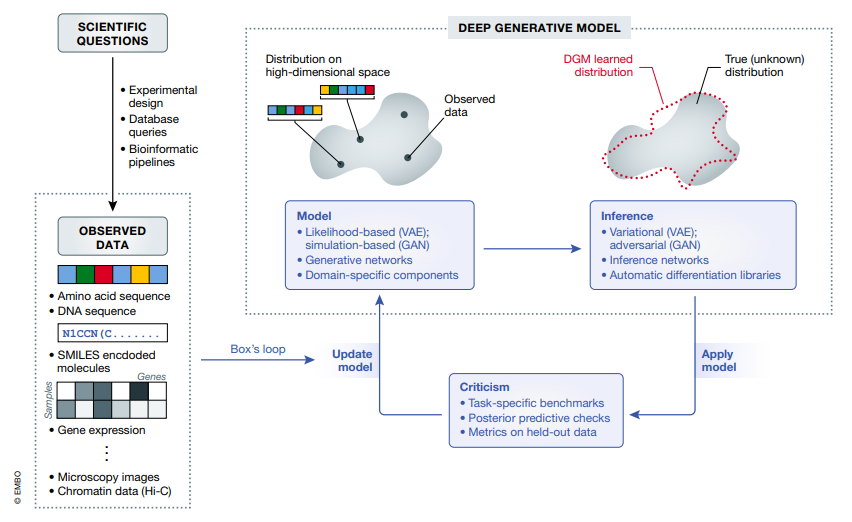
\includegraphics[height=65mm, width=105mm]{dbm}
\end{figure}
\end{frame}

\begin{frame}{A recent VAE for transcriptomics data: scV1}

\end{frame}


\begin{frame}{Recent improvements of interpretability}

\begin{figure}
\begin{center}
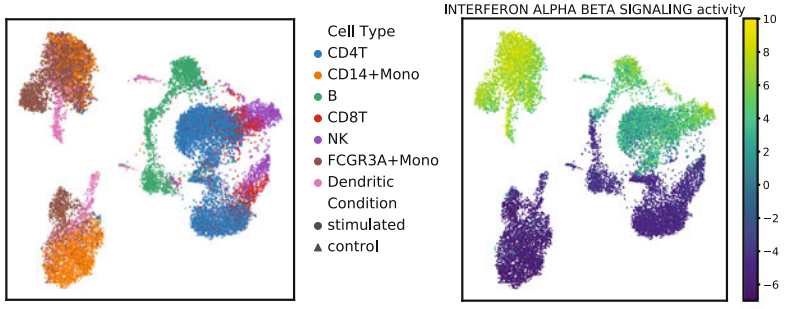
\includegraphics[width=1.0\textwidth]{immune}
\end{center}
\caption{Phenotype segregation using a VAE on single-cell transcriptomics data. Taken from Seninge et al.}
\end{figure}

\end{frame}




\section{References}

% Adding the option 'allowframebreaks' allows the contents of the slide to be expanded in more than one slide.
\begin{frame}[allowframebreaks]{References}
	\tiny\bibliography{references}
	\bibliographystyle{apalike}
\end{frame}

\end{document}